\chapter{Prediction of Biological Age}
\label{ch:methylation}

Enough painting. \marginnote{\textbf{\textsf{Download the methylation data set from \url{http://file.biolab.si/datasets/methylation.pkl.gz.} Predictions of age from methylation profile were investigated by Horvath (2013) Genome Biology 14:R115.}}} Now for the real data. We will use a data set that includes human tissues from subjects of different ages. The tissues were profiled by measurements of DNA methylation, a mechanism for cells to regulate gene expression. Methylation of DNA is scarce when we are young and gets more abundant as we age. We have prepared a data set where the degree of methylation was expressed per gene. Let us test if we can predict the age from the methylation profile - and if we can do this better than by just predicting the average age of subjects in the training set.

\begin{figure}[h]
    \centering
    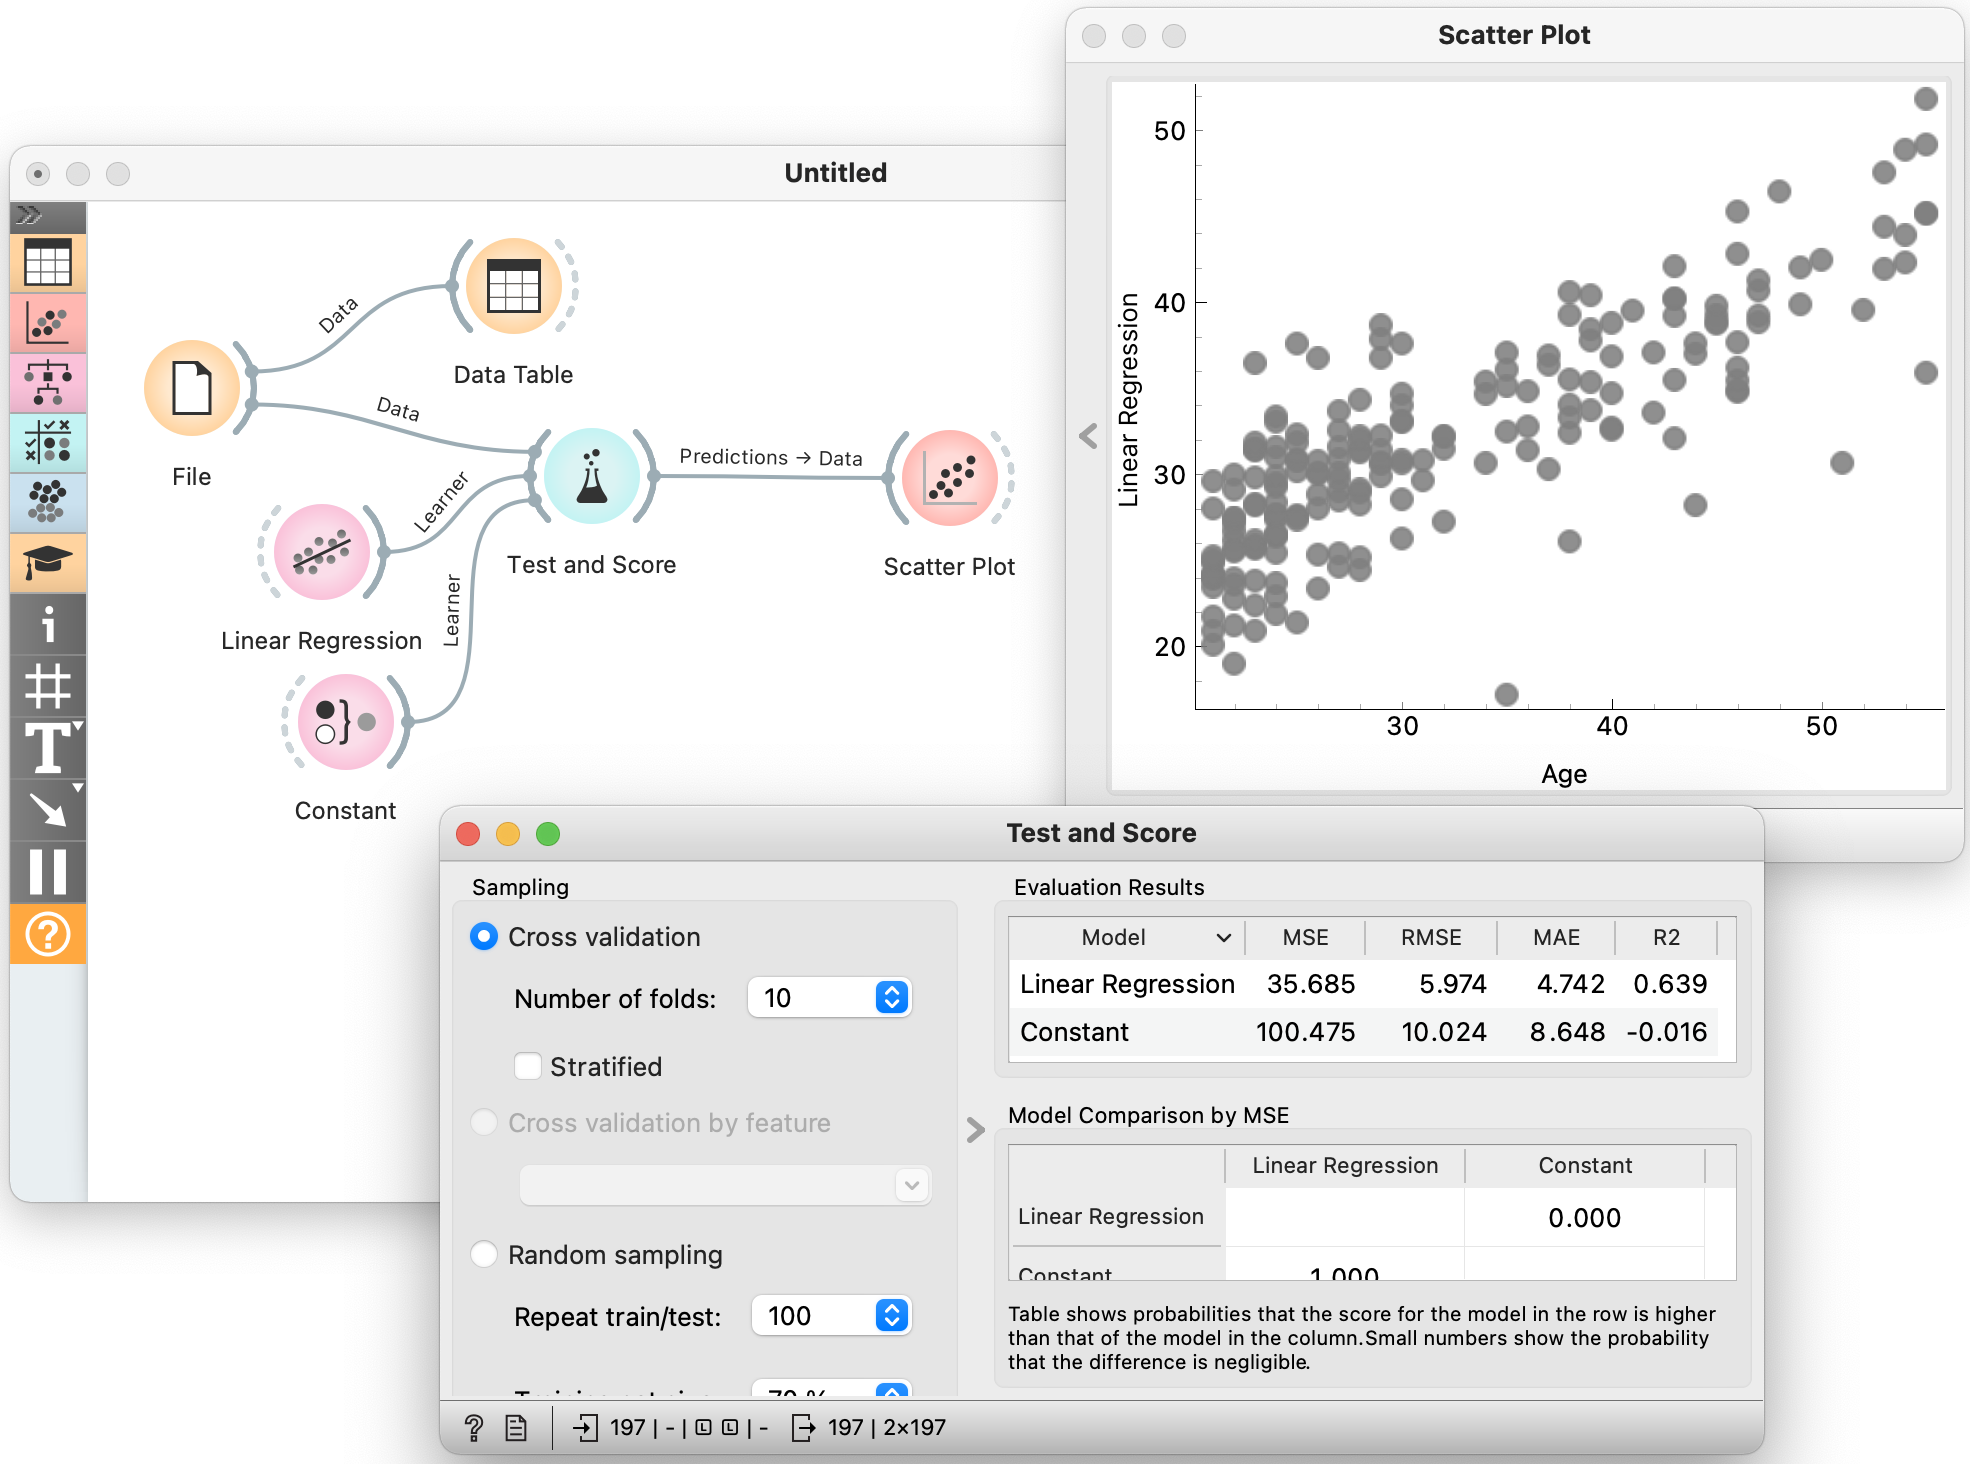
\includegraphics[scale=0.35]{methylation.png}
    \caption{$\;$}
\end{figure}

This workflow looks familiar and is similar to those for classification problems—-the \widget{Test and Score} widget reports on statistics we have not seen before.\marginnote{\textbf{\textsf{Using other learners, like random forests, takes a while on this data set. But you may try to sample the features, obtain a smaller data set, and try various regression learners.}}} MAE, for one, is the mean average error. As for classification, we have used cross-validation. Mean average error was computed only on the test data instances and averaged across ten cross-validation runs. The results indicate that our modeling technique misses the age by about five years, which is a much better result than predicted by the mean age in the training set.